\documentclass{report}
\usepackage[margin=1in, paperwidth=8.5in, paperheight=11in]{geometry}
%Math packages%
\usepackage{amsmath}
\usepackage{amsthm}
%% for hyperlinks
\usepackage{url}
\usepackage[colorlinks=true,linkcolor=cyan]{hyperref}

%Spacing%
\usepackage{setspace}
\onehalfspacing
%Lecture number%
\newcommand{\lectureNum}{7}
%Variables - Date and Course%
\newcommand{\curDate}{January 24, 2017}
\newcommand{\course}{CS 240}
%Defining the example tag%
%\theoremstyle{definition}%
\newtheorem{ex}{Example}[section]
%Setting counter given the lecture number%
\setcounter{chapter}{\lectureNum{}}
%Package to insert code%
\usepackage{listings}
\usepackage{courier}
\usepackage{xcolor}
\lstset { 
    tabsize=2,
    breaklines=true,
    language=C++,
    backgroundcolor=\color{blue!8}, % set backgroundcolor
    basicstyle=\footnotesize\ttfamily,% basic font setting
}
%Package to draw trees%
\usepackage{tikz}

\begin{document}
%Note title%
\begin{center}
\begin{Large}
\textsc{\course{} | Lecture \lectureNum{}}
\end{Large}
\end{center} 
\noindent \textit{Bartosz Antczak} \hfill
\textit{Instructor: Eric Schost} \hfill
\textit{\curDate{}}
\rule{\textwidth}{0.4pt}

% Actual Notes%
\section{Randomized Algorithms}
A \textbf{randomized algorithm} is an algorithm with such an implementation that relies on generating random numbers in addition to the input.
There exist several kinds of such algorithms. In this course, we will see {\bf Las Vegas} algorithms, whose output is 
always correct, and which are ``probably fast'' (the runtime is given in expectation). Another class of randomized 
algorithms are {\bf Monte Carlo} algorithms, which are always fast and ``probably correct'' (the output 
may be incorrect, with a small probability).\\


Note that computers \textit{can't actually generate} random
numbers. The generated number always depends on some external factors,
such as the system clock most notably. Using these external sources is
expensive, so instead we use a \textit{pseudo-random number generator}
(PRNG), which is a deterministic program that uses a true-random
initial value or \underline{seed}. This approach is faster than the
other method. A widely used PRNG is the {\it Mersenne twister}; 
wikipedia has the example of a C++ implementation of it at
\url{https://en.wikipedia.org/wiki/Mersenne_Twister#C.2FC.2B.2B_implementation}.



\subsection{Expected Running Time}
The expected running time, denoted $T^{(\mathrm{exp})}(I)$, of a randomized algorithm for a particular input $I$ and a sequence of random numbers $R$ is
$$T^{(\mathrm{exp})}(I) = E[T(I,R)] = \sum_{R} T(I, R) \cdot \mathrm{Pr}[R]$$
(Pr[$R$] denotes is the probability of getting the particular value in $R$). Note that the expected runtime is defined as \textit{expected} because it considers the statistical probability of $R$.\\
%exp is just expected%
For randomized algorithms, the best-, worst-case scenario are often at about the same running time.
\subsection{Randomized QuickSelect}
How would we want to randomize the quick select algorithm?
\subsubsection{First Method}
Randomly permute the input (an array \texttt{A}) first using shuffle.
\begin{lstlisting}
shuffle(A) {
	for i = 0 to n - 2 do
		swap(A[i], A[i + random(n-i)]) // random(n) returns an integer from 0 to n-1
}
\end{lstlisting}
(Note: we loop until the second last element in the array to avoid swapping the last element with itself, which is redundant) 
We choose $n-1$ integers; we have $n$ choices for the first one, $n-1$ for the second one, etc;
altogether, this gives us $n!$ different choices, all having the same probability
(we assume that when we call ${\tt random}(i)$, the probability of getting any integer from 0 to $i-1$ is uniform). 
Suppose then that input $A$ represents a permutation of $[1,\dots,n]$. No matter what permutation we take as input, after shuffle, 
all permutations of $[1,\dots,n]$ are equiprobable, and this implies that  the expected cost becomes the same as the average cost, which is $\Theta(n)$. 

However, because the algorithm calls the \texttt{random} function $n$ times, this algorithm is too costly. Let's see a different 
approach. 
\subsubsection{Second Method}
Let's just change the pivot selection.
\begin{lstlisting}
choose-pivot(A) {
	return random(n)
}
\end{lstlisting}
And in our main quick select algorithm
\begin{lstlisting}
quick-select(A, k) {
	p = choose-pivot(A)
	.... // Rest of the original algorithm
}
\end{lstlisting}
With an equal probability for every pivot, there is at least a 50\%
change the pivot has position $\frac{n}{4} \leq i <
\frac{3n}{4}$. This means that half the time, the recursive call is
made in length at most $\frac{3n}{4}$ (reminder: the recursive call is 
in length either $i$ (if $k > i$) or $n-i-1$ (if $k < i$),
and when $\frac{n}{4} \leq i <
\frac{3n}{4}$, both $i$ and $n-i-1$ are less than $\frac{3n}{4}$);
 the other time, we don't really know, so we simply say that the recursive call
is made in length at most $n$. So our expected runtime for this randomized algorithm is:

\begin{align*}
T^{(\mathrm{exp})}(n) &\leq cn+ \frac{1}{2}T^{(\mathrm{exp})}(n) + \frac{1}{2}T^{(\mathrm{exp})}\left(\frac{3n}{4}\right) \\
\frac{1}{2} T^{(\mathrm{exp})}(n) &\leq cn + \frac{1}{2}T^{(\mathrm{exp})}\left(\frac{3n}{4}\right) && \text{(Rearrange)}\\
T^{(\mathrm{exp})}(n) &\leq 2cn + T^{(\mathrm{exp})}\left(\frac{3n}{4}\right) && \text{(Multiply by 2)}
\end{align*}
The result implies that $T^{(\mathrm{exp})} \in O(n)$, just like the first method. \textbf{This is generally the fastest quick-select implementation}. This implementation is less costly because we only call \texttt{random} $\log n$ times, rather than $n$ times.
\subsubsection{Worst-case Linear Time}
In 1973, the ``medians-of-five" algorithm was created for pivot selection. We use the following 
algorithm for finding our pivot.
\begin{enumerate}
\item Split the array (of length $n$) into $\frac{n}{5}$ subsets $B_1,\dots,B_{n/5}$. This causes each subset $B_i$ to have a length of 5.
  For example, if 
$$A=[3,10,17,1,20,1,2,4,20,10,12,22,13,1,4,7,19,13,15,2,18,3,7,1,2],$$
we have $n=25$, and 
\begin{align*}
  B_1&=[3,10,17,1,20] \\
  B_2&=[1,2,4,20,10] \\
  B_3&=[12,22,13,1,4] \\
  B_4&=[7,19,13,15,2] \\
  B_5&=[18,3,7,1,2]
\end{align*}
\item Find the median $m_i$ of each $B_i$ (i.e., if the subset is $B_1 = [3, 10, 17, 1, 20]$, then the median $m_1$ is 10). This step has a runtime of $\frac{n}{5} \times c \in O(n)$, where $c$ is the time to calculate the median of a set like $B_i$, which is constant since each array has length 5.
\item Return the median $m$ out of the $\frac{n}{5}$ calculated medians (by calling quickselect)
\end{enumerate}
For the example above, we have $[m_1,m_2,m_3,m_4,m_5] =
[10,4,12,13,3]$, so we return $m=10$. 
Let us see why this algorithm has a runtime of $\Theta(n)$. We use two facts:
\begin{itemize}
\item If a function $f(n)$ satisfies the sloppy recurrence $f(n) \le k n + f(\alpha n) + f(\beta n)$,
  for some constants $k,a,b$ such that $a+b < 1$, then $f(n)$ is $O(n)$. 
\item There are at most $7n/10$ elements in $A$ less than (or equal to) $m$, and 
  at most $7n/10$ elements in $A$ greater than (or equal to) $m$ (this means that $m$ is not 
  too far from the actual median of $A$).

  We can prove the first claim as follows (the other one works the
  same): $m$ is the median of $m_1,\dots,m_{n/5}$, so half of the
  $m_i$'s are greater than or equal to $m$. For each of these $m_i$'s,
  there are $3$ elements in $B_i$ that are greater than or equal to
  $m_i$, because $m_i$ is the median of the 5-element set
  $B_i$. Altogether, there are {\em at least} $1/2 \times n/5 \times 3
  = 3n/10$ elements in $A$ greater than or equal to $m$; as a result,
  there are {\em at most} $n-3n/10=7n/10$ elements in $A$ less than or
  equal to $m$.
\end{itemize}

Let us call $T_{P}(n)$ the runtime of this algorithm for finding the
pivot, and $T_{QS}(n)$ the runtime of quickselect using this
pivot. The pivot algorithm spends $O(n)$ to find the $m_i$'s and call
quickselect in length $n/5$, so $T_P(n) = cn + T_{QS}(n/5)$.
Quickselect calls the pivot algorithm in length $n$, spends $O(n)$ for
partition, and does a recursive call in length at most $7n/10$ (by the
second item above), so $T_{QS}(n) \le c'n + T_P(n) +
T_{QS}(7n/10)$. Putting these two relations together, we get
$T_{QS}(n) \le (c+c') n + T_{QS}(n/5)+ T_{QS}(7n/10)$. Since 
$1/5 + 7/10 = 9/10 < 1$, the first item above implies that $T_{QS}(n)$ 
is in $O(n)$.

We could write the same algorithm using a subdivision of $A$ into 
$n/3$ subsets of lenth 3. All calculations done, we would end up 
with the recursion $T_{QS}(n) \le (c+c') n + T_{QS}(n/3)+ T_{QS}(2n/3)$,
but because $1/3 + 2/3 =1$, this does not imply a linear runtime
(in this case, $T_{QS}(n) \in O(n\log(n))$).




\section{The QuickSort Algorithm}
The quick sort algorithm is based on a sorting method developed by Hoare in 1960. On input array \texttt{A} of size \texttt{n}:
\begin{lstlisting}
quick-sort1(A) {
	if (n <= 1) return
	p = choose-pivot(A)
	i = partition
	quick-sort1(A[0, 1, ..., i-1])
	quick-sort1(A[i+1, ..., n-1])
}
\end{lstlisting}
Analysing the algorithm, the worst case runtime occurs when one array always has size $n-1$ and the other has size 0:
$$T^{\mathrm{(worst)}}(n) = T^{\mathrm{(worst)}}(n-1) + \Theta(n) \in \Theta(n^2)$$
The best case runtime occurs when both arrays are split evenly on each recursive call
$$T^{\mathrm{(best)}}(n) = T^{\mathrm{(best)}}\left(\left\lfloor \frac{n-1}{2}\right\rfloor\right) + T^{\mathrm{(best)}}\left(\left\lceil \frac{n-1}{2}\right\rceil\right) + \Theta(n) \in \Theta(n \log n)$$
We can visualize these runtime using a tree (a the height of the tree shows the how deep the recursive calls go).\\

The worst-case runtime splits the array into sizes $n-1$ and 0 (i.e., it has a height of $n$):
%WORST CASE%
\begin{center}
\begin{tikzpicture}[
  level distance=40 pt,
  every node/.style={circle,draw},
  level 1/.style={sibling distance=60 pt},
  level 2/.style={sibling distance=60 pt},
  level 3/.style={sibling distance=60 pt},
  level 4/.style={sibling distance=60 pt},
  level 5/.style={sibling distance=60 pt}
]
  \node {$n$}
    child [missing]
    child {node {$n-1$}
      child [missing]
      child {node {$n-2$}
      	child[missing]
      	child {node {$\cdots$}
      		child [missing]
      		child {node {1}}}}
    };
\end{tikzpicture}
\end{center}
The best case runtime splits the arrays evenly, or off by at most 1 (i.e., has a height of $\log n$)
\begin{center}
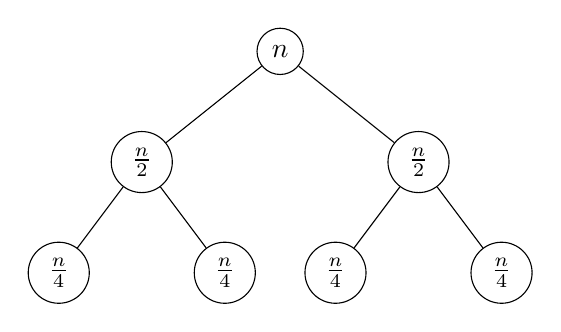
\begin{tikzpicture}[
  level distance=40 pt,
  every node/.style={circle,draw},
  level 1/.style={sibling distance=100 pt},
  level 2/.style={sibling distance=60 pt},
  level 3/.style={sibling distance=60 pt},
  level 4/.style={sibling distance=60 pt},
  level 5/.style={sibling distance=60 pt}
]
  \node {$n$}
    child {node {$\frac{n}{2}$}
    	child {node {$\frac{n}{4}$}}
    	child {node {$\frac{n}{4}$}}}
    child {node {$\frac{n}{2}$}
    	child {node {$\frac{n}{4}$}}
    	child {node {$\frac{n}{4}$}}};
\end{tikzpicture}
\end{center}

\subsubsection{Average-case Analysis of Quick Sort}
By our previous remark, we observe that the runtime is determined by the height $H$ of the tree that defines the depth of the recursive calls.
Precisely, for an input array of length $A$, let us write
$T(A)$ for the runtime of quicksort on input $A$, and $H(A)$ for the depth of the recursion.
Then, we have $T(A) = O(n H(A))$, since the total work spent at any level of the recursion
tree is $O(n)$, and there are $H(A)$ such levels.

Our goal is to estimate the average runtime $T(n)$, defined as 
$$T(n) = \frac 1{n!} \sum_{\text{$A$ permutation of $[1,\dots,n]$}} T(A).$$
Because of the relation $T(A) = O(n H(A))$, we get $T(n) = O(n H(n))$,
where $H(n)$ is the average depth of the recursion:
$$H(n) = \frac 1{n!} \sum_{\text{$A$ permutation of $[1,\dots,n]$}} H(A).$$
We now prove that $H(n)$ is in $O(\log(n))$, which implies that 
$T(n)$ is in $O(n \log(n))$.

The details of the proof are similar to what we did for quickselect.
({\'E.S.}: you do not need to know them).
We call $i$ the position of the pivot, and we define 
$$H(n,i) = \frac 1{(n-1)!} \sum_{\text{$A$ permutation of $[1,\dots,n]$ with pivot position $i$}} H(A).$$
Because all pivot position are equiprobable, we get 
\begin{equation}\label{eq:HnHni}
H(n) = \frac 1n \sum_{i=0}^{n-1} H(n,i).  
\end{equation}
Let us rewrite the sum giving $H(n,i)$. We know that for any binary tree $T$,
with children $T'$, $T''$, we have the equality
$\text{height}(T) \le 1 + \max(\text{height}(T'),\text{height}(T'')),$
which implies $\text{height}(T) \le 1 +\text{height}(T')$ and 
 $\text{height}(T) \le 1 +\text{height}(T'')$. As result,
we get 
$$H(n,i) \le  1 + \frac 1{(n-1)!} \sum_{\text{$A$ permutation of $[1,\dots,n]$ with pivot position $i$}} 
        H(\text{left side of the recursion})$$
and
$$H(n,i) \le  1 + \frac 1{(n-1)!} \sum_{\text{$A$ permutation of $[1,\dots,n]$ with pivot position $i$}} 
        H(\text{right side of the recursion}).$$
One can see without much trouble that in the first equation, the average is simply $H(i)$, 
and that it becomes $H(n-i-1)$ in the second one. This gives us
$$H(n,i) \le 1 + H(i) \quad\text{and}\quad H(n,i) \le 1 + H(n-i-1).$$
Plugging this in~\eqref{eq:HnHni}, we deduce
$$H(n) \le 1 + \frac 1n \sum_{i=0}^{n-1} \max(H(i), H(n-i-1)).$$
We finish as before by a case discussion:
\begin{itemize}
\item if $i < n/4$ or $i \ge 3n/4$, we use the upper bound 
  $\max(H(i), H(n-i-1)) \le H(n)$. There are $n/2$ such cases.
\item if $n/4 \le i < 3n/4$, $\max(H(i), H(n-i-1)) \le H(3n/4)$. There
  are $n/2$ such cases as well.
\end{itemize}
This gives us the inequality 
$$H(n) \le 1 + \frac 12 H(n) + \frac 12 H(3n/4).$$
After rearrange and multiplying by 2 (as we did for quickselect), 
we get 
$$H(n) \le 2 + H(3n/4).$$
Unroll the recurrence:
$$H(n) \le 2 + H( (3/4) n) \le 2 + 2 + H((3/4)^n) \le 2 + 2 + 2 + H((3/4)^3 n) \le \cdots$$
The number of terms in the sum is $O(\log(n))$, so $H(n) \in O(n)$, as claimed.

QuickSort is often the most efficient algorithm in practice.
%END%
\end{document}
